\documentclass[11pt,a4paper]{scrartcl}

\usepackage[a4paper, total={6in, 8in}]{geometry}

\usepackage[utf8]{inputenc}
\usepackage[T1]{fontenc}
\usepackage[english]{babel}
\usepackage[babel,german=quotes]{csquotes}
\usepackage[pdftex]{graphicx}
\usepackage{amsmath,amssymb,amsthm}
\usepackage{latexsym}
\usepackage{hyperref}
\usepackage{import}

\newcommand{\Fig}[0]{Fig.}
\newcommand{\Eq}[0]{Eq.}

\hypersetup{
	pdftitle={CNN for plot function detection},
	pdfsubject={Applied Machine Learning Group Project},
	pdfauthor={Philipp Fürst},
	pdfkeywords={wissenschaftliches Schreiben}
}
\usepackage[anythingbreaks]{breakurl}
\usepackage{listings}
\lstset{numbers=left,
	numberstyle=\small,
	numbersep=5pt,
	breaklines=true,
	showstringspaces=false,
	frame=1 ,
	xleftmargin=15pt,
	xrightmargin=15pt,
	basicstyle=\ttfamily\scriptsize,
	stepnumber=1,
	keywordstyle=\color{ao}\textbf,         
  	commentstyle=\color{gray},       
  	stringstyle=\color{mauve}         
}
\lstloadlanguages{TeX}

\usepackage{color}
\definecolor{ao}{rgb}{0.0,0.0,1.0}
\definecolor{dkgreen}{rgb}{0,0.6,0}
\definecolor{gray}{rgb}{0.5,0.5,0.5}
\definecolor{lightgray}{rgb}{0.8,0.8,0.8}
\definecolor{mauve}{rgb}{0.58,0,0.82}

\usepackage[backend=biber]{biblatex} 
\ExecuteBibliographyOptions{
sorting=nyt, 
bibwarn=true, 
isbn=false, 
url=false 
}
\addbibresource{literatur.bib} 

\setlength{\topmargin}{-10mm}

\begin{document}
	\lstset{language=tex}
	
	\pagenumbering{roman}
	\pdfbookmark{Title page}{titlepage}
	\begin{titlepage}
		 \center
		 
\includegraphics[scale=0.2]{ImageFiles/unistuttgart_logo_de} 
		 \vspace*{2cm} 
		
		\begin{center} \large 
		     
			 \vspace*{2cm}
			 {\huge \textbf{CNN for plot function detection}}
			 \vspace*{2.5cm}
			
			 Applied Machine Learning Group Project
			 \vspace*{2.5cm}
			
			 Philipp Fürst (3383656)\\
			 Wasim Essbai (3649361)
			 \vspace*{1cm}
		\end{center}
	\end{titlepage}

	\tableofcontents
	\listoffigures
	\listoftables
	\pagebreak
	
	\pagenumbering{arabic}
  	\pagestyle{plain}
  
	\section{Introduction}
	The aim of this project is to design a machine learning model able to recognize a mathematical function from its graph. This is showed in \Fig~\ref{fig:GeneralIdea}.
	\begin{figure}[h!]
		\centering
		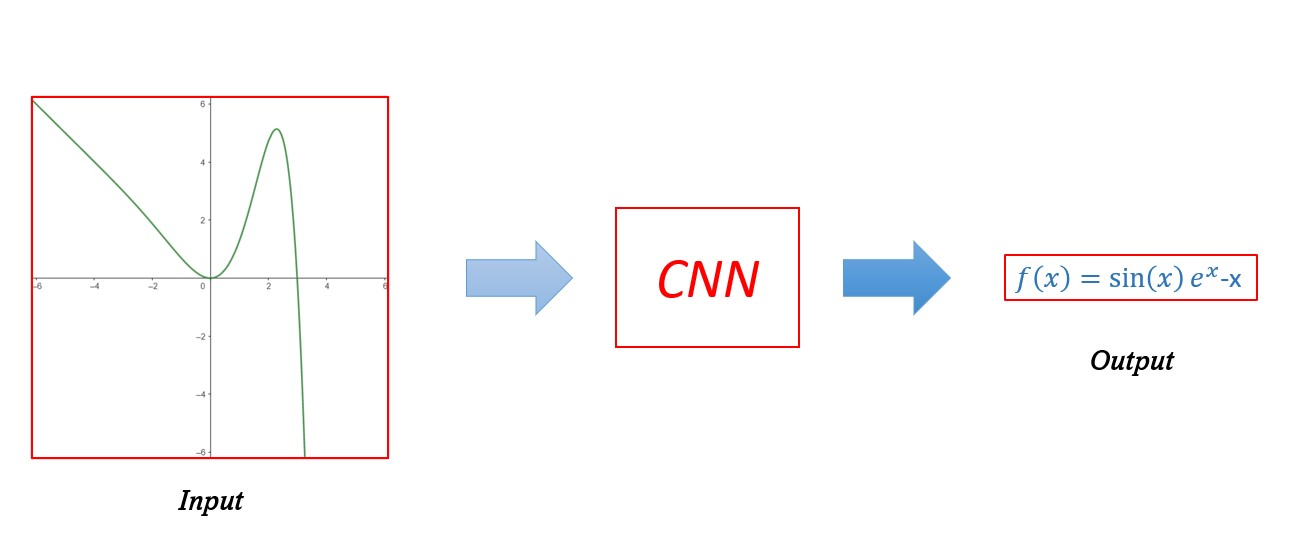
\includegraphics[width=0.7\linewidth]{./ImageFiles/general_idea}
		\caption{Final result to achieve}
		\label{fig:GeneralIdea}
	\end{figure}\\This problem can be approached as an image classification task.A common method for solving this type of problem is to use Convolutional Neural Networks (CNN).

	\section{Data Generation}
	Neural Networks models need a large amount of training data. The first challenge was to retrieve that data.\\
	For this project we developed an algorithm to generate and classify data, since no graph function datasets were available. This algorithm allowed to retrieve an arbitrary large amount of data. It is described in the following section.
	
	\import{./TextFiles/Data Generation/}{Algorithm.tex}
	\import{./TextFiles/Data Generation/}{Plots.tex}
	\import{./TextFiles/Data Generation/}{Labeling.tex}


	\section{CNN model}
	\import{./TextFiles/CNN/}{Architecture.tex}
	\import{./TextFiles/CNN/}{Implementation.tex}
	
	\section{Training}
	First we created a smaller data set consisting of 2000 function plots and the corresponding function vectors. This was again split into 70\% training data, 15\% validation data and 15\% test data. Based on this we tested different sizes of kernels, epochs and learning rates, as there the execution time remained manageable.\\
	We achieved the highest performance with 2x2 kernels, padding of the first two convolutional layers, 15 epochs, 0.1\% learning rate, and a scaling factor of 1000000, which further separates the closely spaced numbers of vector entries, allowing easier learning of the entries.\\
	With these parameters found, we could train the CNN on our large dataset (50000). The execution of the training was done GPU-based on Google Colab.

	\section{Experimental Results}
	\textcolor{red}{learning curve of loss over epochs and accuracy over epochs, for full vector length and not full vector length (both on the big data set)}

	\section{Conclusions}
	Our general idea works. It is possible to recognize functions from a given plot and to classify their mathematical function using our trained CNN. The performance is still improvable.\\
	Among other things, this is due to the fact that there are redundancies within our data sets, which are currently not filtered out. For example, one and the same function can be generated by different mathematical functions \(f(x) = |x^2| = x^2\). Eliminating these would be a first step to have a more meaningful dataset.\\
	Additionally, due to lack of computer resources, we trained our CNN on only 50000 samples. This is very small in the dimension of machine learning and therefore still expandable. However, the approach is promising if already with these small data sets accuracies of \textcolor{red}{X.XX\%} are achieved when comparing all but one vector entries of the mathematical function. 

\end{document}